\appendixchapter{\FModel{}}

\subsection*{Graphical Representation: The \forcediag{}}

\textbf{Example:} A finger pushing a box over a surface at a constant speed.

%\vspace{-1cm}
\begin{figure}[h!]
	\centering
	\begin{subfigure}[t]{0.45\textwidth}
		\centering
		\caption*{\textbf{Picture of the situation}}
		\begin{tikzpicture}[thin,scale=0.9, every node/.style={transform shape},background rectangle/.style={fill=white}, show background rectangle]
			%Finger
			\node[xscale=-1,inner sep=0pt,rotate=45] (finger) at (1,1) {
\includegraphics[width=2cm]{finger.eps}};

			% Surface
			\draw (0,0) -- (5,0);
			\foreach \x in {0.5,1,1.5,2,2.5,3,3.5,4,4.5,5}
    				\draw (\x,0) -- (\x-0.25,-0.25);
			
			%Box
			\draw (2.5,0) rectangle (4.5,2) node[midway] {Box};
		\end{tikzpicture}
		\caption*{}
	\end{subfigure}
	\hspace{0.05\textwidth}
	\begin{subfigure}[t]{0.45\textwidth}
		\centering
		\caption*{\textbf{\forcediag{}}}
		\begin{tikzpicture}[thin,scale=0.9, every node/.style={transform shape},background rectangle/.style={fill=white}, show background rectangle]
			% draw object node
			\draw (0,0) node[circle,minimum size=6pt,fill,inner sep=1pt]{} node[left=6pt]{Box};	
			
			% draw and label F1
			\draw[-{Stealth[scale=1.2]}, line width=1pt] (0,0) -- (0,1.5) node[right=3pt,align=center] {$\vec{F}_\text{Surface on Box}$};
			% draw and label F2
			\draw[-{Stealth[scale=1.2]}, line width=1pt] (0,0) -- (0,-1.5) node[right=3pt,align=center] {$\vec{F}_\text{Earth on Box}$};
			% draw and label F3
			\draw[-{Stealth[scale=1.2]}, line width=1pt] (0,0) -- (2,0) node[right=3pt,align=center] {$\vec{F}_\text{Finger on Box}$};
		\end{tikzpicture}
		\caption*{}
	\end{subfigure}
\end{figure}

      \vspace{-5mm}
      \begin{wrapfigure}[3]{r}{5cm}
        \centering
        \vspace{-\baselineskip}
			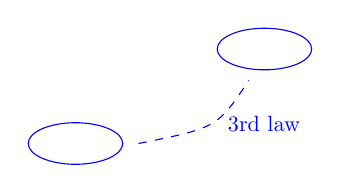
\begin{tikzpicture}[scale=.8, every node/.style={transform shape}]{r}{1}
				\draw[blue] (0,0) ellipse (0.75cm and 0.33cm);
				\draw[blue] (3,1.5) ellipse (0.75cm and 0.33cm);
				\draw[blue,dashed] (1,0) .. controls (2.25,0.25) .. (2.75,1) node[midway, right=4pt, blue] {3rd law};
			\end{tikzpicture}
	  \end{wrapfigure}

	\noindent To identify which forces are part of a 3rd law pair, draw a \forcediag{} for \emph{each} of the two interacting objects, circle the corresponding arrows, and connect the circles with a line:
	
\vspace{1cm}

\subsection*{Algebraic Representations:}

\subsubsection*{\textit{Newton's Three Laws of Motion}}

\begin{enumerate}[I.]
	\item Without a net force, there can be no change in the velocity of an object:
	
	\begin{center}\framebox[1.1\width][c]{If $\sum\vec{F}=0$, then $\Delta\vec{v}=0$.}\end{center}
	
	\item An object will be accelerated if there is a net force acting upon it:
	
	\begin{center}\framebox[1.1\width][c]{$\sum\vec{F}=m\vec{a}$}\end{center}

	\item If object $A$ exerts a force on object $B$, object $B$ \emph{simultaneously} exerts an equal and opposite force on object $A$:
	
	\begin{center}\framebox[1.1\width][c]{$\vec{F}_\text{A on B} = -\vec{F}_\text{B on A}$}\end{center}
	
\end{enumerate}

\subsubsection*{Relation of a net force to momentum and work:}

\begin{align*}
	\text{Net Impulse imparted on a system:}			&& \sum\vec{I} &= \sum\vec{F}_\text{avg. ext.} \cdot \Delta t = \Delta \vec{p}\\[5mm] 
	\text{Work done on a system:}	&& W &= \sum F_\text{avg. ext.} \cdot d_\text{parallel to net force}
\end{align*}

\null